% =============================================================================
% AIMoodDiary -- Project report (Overleaf)
% ---------------------------------------------------------------------------
% STYLING: Navy + gold palette (MM* colors), tcolorbox abstract/callouts, fancy
%   headers, colored section numbers, titletoc, microtype, 1.08 line spread.
% FONTS: pdflatex + Latin Modern (lmodern). Replace with XCharter/TeX Gyre
%   if you prefer a book-like serif: e.g. \usepackage{XCharter} after fontenc.
% SETUP: Create folder ``figures/'' in Overleaf. For each figure slot below:
%   (1) Add the named PNG to figures/
%   (2) Remove the \% at the start of the \includegraphics line (uncomment it)
%   (3) Delete the whole brown ``PENDING'' tcolorbox under that line (and these
%       instruction comments if you like). Recompile.
% TWEAK: Title/author in ``Document title block'' below.
% FIGURE FILES (copy into Overleaf project folder figures/):
%   app-01-home.png app-02-dashboard.png app-03-quickcheck.png app-04-diary.png
%   app-05-history.png app-06-insights-trend.png app-07-insights-calendar.png
%   app-08-reflect-hub.png app-09-reflect-mood.png app-10-unwind.png
%   legacy-01-streamlit.png legacy-02-confusion-3cl.png legacy-03-emotion-distribution.png
% =============================================================================

\documentclass[11pt,a4paper]{article}

\usepackage[utf8]{inputenc}
\usepackage[T1]{fontenc}
\usepackage{lmodern}
% fancyhdr: avoid "headheight is too small" (needs ~22pt for two-line header area)
\usepackage[margin=2.2cm,headheight=22pt,headsep=0.4cm,bottom=2.3cm]{geometry}
\usepackage{amsmath,amssymb}
\usepackage{booktabs}
\usepackage{tabularx}
\usepackage{graphicx}
\usepackage{xcolor}
\usepackage{microtype}
\usepackage{setspace}
\setstretch{1.08}

% --- Color palette (aligns with a calm “wellness + tech” feel) -------------
\definecolor{MMnavy}{HTML}{1E3A5F}
\definecolor{MMnavyL}{HTML}{2C5282}
\definecolor{MMgold}{HTML}{C9A227}
\definecolor{MMgoldL}{HTML}{E8D48A}
\definecolor{MMsurface}{HTML}{F7F5F0}
\definecolor{MMrule}{HTML}{C8C4BC}
\definecolor{codebg}{HTML}{F4F2ED}
\definecolor{codeframe}{HTML}{D8D4CC}

% --- tcolorbox (abstract, notes, code frames, figure placeholders) ----------
\usepackage[most,skins,breakable]{tcolorbox}
\tcbuselibrary{listings}
\usepackage{titlesec}
\usepackage{titletoc}
\usepackage{enumitem}
\usepackage{float}
\usepackage{caption}
\usepackage{subcaption}
\usepackage{fancyhdr}
\usepackage{lastpage}
\usepackage{tikz}
\usetikzlibrary{positioning,arrows.meta}

% --- Listings: improved readability -----------------------------------------
\usepackage{listings}
\definecolor{kw}{HTML}{0D6E9E}
\definecolor{str}{HTML}{2E7D32}
\definecolor{cmnt}{HTML}{6D6D6D}

\lstdefinestyle{mmcode}{
  language=Python,
  basicstyle=\ttfamily\footnotesize\linespread{0.95}\selectfont,
  keywordstyle=\color{kw}\bfseries,
  commentstyle=\color{cmnt}\itshape,
  stringstyle=\color{str},
  numberstyle=\tiny\color{cmnt},
  numbersep=6pt,
  showstringspaces=false,
  breaklines=true,
  breakatwhitespace=true,
  tabsize=4,
  xleftmargin=0.4em,
  xrightmargin=0.3em,
  frame=none,
  backgroundcolor=\color{codebg},
  columns=fullflexible,
  keepspaces=true,
}
\lstset{style=mmcode, literate={—}{{---}}1 {–}{{-}}1, columns=fullflexible }
% Extra line stretch to reduce overfull hboxes (tighter than \sloppy for whole doc)
\setlength{\emergencystretch}{2.5em}
\lstdefinelanguage{json}{
  sensitive=false,
  morestring=[b]",
}
\newcommand{\CodeFilename}[1]{\vspace{-0.25em}\begin{center}\scriptsize\color{MMnavyL!80!black}\textsf{[\,#1\,]}\end{center}\vspace{-0.2em}}

% --- Hyperref + better URL line breaks in PDF --------------------------------
\usepackage{hyperref}
\usepackage{xurl}
\hypersetup{
  colorlinks=true,
  linkcolor=MMnavyL,
  urlcolor=MMnavyL,
  citecolor=MMnavyL,
  pdfauthor={Manu Mathew Jiss, Pramod Gupta},
  pdftitle={AIMoodDiary: GoEmotions, deployed journaling, hybrid inference},
  bookmarksopen=true
}

% --- Section and TOC styling (numbered sections) ----------------------------
\titlecontents{section}
  [0.9em] {}
  {\bfseries\color{MMnavy!85!black} \thecontentslabel.\hspace{0.55em}}
  {}
  {\hfill\color{MMnavy!50}\contentspage}[\vspace{2pt}]

% Section: numbered badge + underline (no explicit package)
\titleformat{\section}
  {\bfseries\Large\color{MMnavy}}
  {\fcolorbox{MMnavy!32}{MMnavy!6}{\sffamily\strut\thesection}}
  {0.55em}
  {}
  [\vspace{0.1em}\begingroup\color{MMrule}\hrule height 0.55pt\endgroup]

\titleformat{\subsection}
  {\bfseries\large\color{MMnavyL}}
  {\thesubsection}
  {0.45em}
  {}

\titlespacing*{\section}{0pt}{1.6em plus 0.2em minus 0.1em}{0.85em}
\titlespacing*{\subsection}{0pt}{1.1em}{0.45em}

% --- Page headers / footers -------------------------------------------------
\pagestyle{fancy}
\fancyhf{}
\renewcommand{\headrulewidth}{0.4pt}
\renewcommand{\headrule}{\hbox to\headwidth{\color{MMrule}\leaders\hrule height \headrulewidth\hfill}}
\fancyhead[L]{\small\sffamily\color{MMnavyL!85}AIMoodDiary}
\fancyhead[R]{\small\sffamily\color{MMnavyL!85}Technical report}
\fancyfoot[C]{\small\sffamily\color{MMnavyL!70}Page \thepage\ of \pageref{LastPage}}
% First page: no header clutter
\fancypagestyle{firststyle}{
  \fancyhf{}
  \renewcommand{\headrulewidth}{0pt}
  \fancyfoot[C]{\small\sffamily\color{MMnavyL!70}Page \thepage\ of \pageref{LastPage}}
}
\captionsetup{
  font=small,
  labelfont={bf,sf,color=MMnavyL},
  textfont=it,
  margin=1.2em,
  skip=0.55em
}
\captionsetup[sub]{font=footnotesize,labelformat=simple}

% --- tcolorbox helpers ------------------------------------------------------
\newtcolorbox{CalloutNote}[1]{colback=MMgoldL!18,colframe=MMgold!55,
  leftrule=4pt,rightrule=0.5pt,toprule=0.5pt,bottomrule=0.5pt,arc=1.2pt,
  title={\sffamily\bfseries\color{MMnavy}#1}, coltitle=MMnavy, colbacktitle=MMgold!25}

% Placeholder for figures: softer than \fbox
\newtcolorbox{FigPlaceholder}[1][]{colback=MMsurface,colframe=MMrule,arc=1.2pt,
  boxrule=0.6pt, halign=flush center, left=2mm, right=2mm, top=4mm, bottom=4mm, #1}

% GitHub URL box
\newtcolorbox{SourceBox}{enhanced, colback=white, colframe=MMnavy!45,
  boxrule=0.9pt, arc=1.5pt, top=1mm, bottom=1mm, left=2mm, right=2mm,
  colbacktitle=MMnavy!8, coltitle=MMnavy, fonttitle=\sffamily\bfseries, title=Repository,
  titlerule=0.4pt, titlerule style={MMnavy!30}}

% Placeholder while figure file is not yet active: delete this box after you
% uncomment the matching \includegraphics line above.
\newcommand{\MMPending}[2]{%
  \begin{tcolorbox}[
    enhanced, colback=MMgoldL!10, colframe=MMgold!60,
    boxrule=0.75pt, arc=1.2pt, left=2mm, right=2mm, top=1.2mm, bottom=1.2mm,
    title={\sffamily\bfseries\footnotesize\color{MMnavy}PENDING (remove me)},
    colbacktitle=MMgold!20, coltitle=MMnavy
  ]
  \sffamily\footnotesize\textbf{Target file:} \texttt{\detokenize{#1}}\\[0.35em]
  \small\color{black!85}#2
  \end{tcolorbox}%
}

% --- Document title block (edit if needed) ------------------------------------
\newcommand{\TheReportTitle}{AIMoodDiary: From GoEmotions-Based Transformer Training to a Deployed Journaling System with LLM Diaries, Hybrid Inference, and Analytics}
\newcommand{\TheReportTitleShort}{AIMoodDiary: Technical report}
% Authors / affiliation
\newcommand{\TheAuthorA}{Manu Mathew Jiss}
\newcommand{\TheAuthorB}{Pramod Gupta}
\newcommand{\TheAffilLong}{Department of Computer Science, University of the Pacific, USA}
\newcommand{\TheEmailA}{\texttt{m\_jiss@u.pacific.edu}}
\newcommand{\TheEmailB}{\texttt{pgupta@pacific.edu}}

\title{%
  \begingroup
  \sffamily\bfseries\color{MMnavy}
  \fontsize{14.2pt}{17pt}\selectfont
  \TheReportTitle\par
  \endgroup
  \vspace{0.65em}
  {\normalsize\sffamily\mdseries\selectfont\color{MMnavyL!90!black}%
   Technical report, user guide, and research notes\par
  }%
}
% Do not use \par / \smallskip inside \author (breaks standard \maketitle)
\author{%
  \sffamily
  \TheAuthorA\qquad\TheAuthorB\\[0.55em]%
  {\small\TheAffilLong}\\[0.45em]%
  {\small\TheEmailA\qquad\TheEmailB}%
}
\date{\sffamily\color{MMnavyL!75}\today}

\begin{document}
\thispagestyle{firststyle}
\maketitle
\thispagestyle{firststyle}

% --- Abstract: framed -------------------------------------------------------
\begin{tcolorbox}[
  enhanced, colback=MMsurface, colframe=MMnavy!30,
  boxrule=0.85pt, arc=2pt, left=5mm, right=5mm, top=3.5mm, bottom=3.5mm,
  title={\sffamily\bfseries\color{MMnavy}Abstract}, coltitle=MMnavy, colbacktitle=MMnavy!7,
  attach boxed title to top left={xshift=3mm, yshift*=-0.2mm--0.2mm},
  titlerule=0pt, fonttitle=\sffamily\bfseries
]
\small\color{black!88}
AIMoodDiary is a full-stack \textbf{student wellness} web application that records mood, classifies text into \textbf{positive / neutral / negative} using a fine-tuned \textbf{RoBERTa} model (3-class), and surfaces \textbf{history}, \textbf{LLM-assisted diary} entries, \textbf{pattern insights}, and supportive \textbf{Reflect / Unwind} features. A parallel \textbf{legacy} research track uses the \textbf{GoEmotions} dataset, baseline and transformer baselines, and a \textbf{Streamlit} demo. The open-source code is on GitHub: \url{https://github.com/manumathewjiss/moodmirror-student-wellness-tracker/tree/main}. The public app is hosted at \url{https://moodmirror-student-wellness-tracker-six.vercel.app} (Vercel).
\end{tcolorbox}
\vspace{0.3em}
\begin{CalloutNote}{About the name}
This document is titled \textbf{\TheReportTitle}; the product name in the app and codebase is \textbf{AIMoodDiary}.
\end{CalloutNote}
\vspace{0.2em}
% Optional (optional-01-cover-hero.png): add file, then remove \% on next line
% \begin{center}\includegraphics[width=0.32\textwidth]{figures/optional-01-cover-hero.png}\end{center}

% --- TOC: compact title -----------------------------------------------------
\begin{tcolorbox}[colback=white,colframe=MMnavy!20,boxrule=0.6pt,arc=1.2pt,left=0mm,right=0mm,top=1mm,bottom=0mm]
{\sffamily\bfseries\color{MMnavy}\large Contents}
\vspace{0.2em}
\tableofcontents
\end{tcolorbox}
\clearpage
\thispagestyle{fancy}

%==============================================================================
\section{Source code and repository}
\label{sec:github}

The complete project (frontend, full backend, \texttt{hf-deploy} bundle, and \texttt{legacy} NLP research) is available at:

\begin{SourceBox}
\centering\url{https://github.com/manumathewjiss/moodmirror-student-wellness-tracker/tree/main}
\end{SourceBox}

\noindent
\textbf{Layout (typical):} \texttt{frontend/} (Next.js), \texttt{backend/} (FastAPI), \texttt{hf-deploy/} (lighter API for Hub-style hosting), \texttt{legacy/} (notebooks, Streamlit, trained model folders, evaluation), \texttt{migrations/} and Alembic for the database. The repository About page describes it as an AI-powered emotional wellness tracker using NLP, LLMs, and interactive mood analytics\footnote{As summarized on the public GitHub repository page.}.

%==============================================================================
\section{How to use the application (end-user guide)}
\label{sec:userguide}

The following steps describe the \textbf{intended} workflow on the deployed site (\texttt{moodmirror-student-wellness-tracker-six.vercel.app}) or any instance you run locally.

\begin{enumerate}[itemsep=0.35em, leftmargin=1.4em, label=\textbf{\sffamily\color{MMnavyL}\arabic*}.]
  \item \textbf{Create an account.} On the home page, use \textbf{Sign up} with a valid \textbf{email} and a \textbf{username} (3--50 characters). The backend registers you via \texttt{POST /auth/register}.
  \item \textbf{Log in.} Use \textbf{Log in} with your \textbf{username} (email is not required for login on this build). The browser stores the username in \texttt{localStorage} so the nav bar shows you as signed in. You are redirected to the \textbf{Dashboard} (\S\ref{sec:ui-figs}, Figure~\ref{fig:app-dashboard}), which links to all main features.
  \item \textbf{Quick Check.} Open \textbf{Quick Check}, paste any short text (how you feel, a sentence about your day), and submit. The app classifies the text, shows \textbf{label}, \textbf{confidence}, and may show per-class \textbf{probabilities}. The entry is saved to your history.
  \item \textbf{Diary.} On \textbf{Diary} you can:
  \begin{itemize}[itemsep=0.25em]
    \item Pick a \textbf{quick mood} (emoji): one-tap with preset keyword phrases, or
    \item Type \textbf{keywords} (up to 10 input boxes) and an optional \textbf{tone} (e.g.\ casual), then \textbf{Generate diary \& save}. The system asks an LLM to write a short first-person entry \emph{only} from your keywords, then combines classifier scores from keywords and generated text. Optional: use the \textbf{microphone} to dictate; audio is sent to the server, transcribed with \textbf{Whisper}, and filled into a keyword field for editing before you save.
  \end{itemize}
  \item \textbf{History.} View a chronological list of past entries: timestamp, source (e.g.\ manual, diary), raw text, generated diary line (if any), label, and confidence.
  \item \textbf{Insights.} After you have a few saved entries, open \textbf{Insights} to see \textbf{charts} (trend line, bars, etc.) and short \textbf{pattern messages} (trend direction, good/bad weekday, volatility, keyword associations, logging streaks). Deeper transition statistics need more entries (see \S\ref{sec:insights-engine}).
  \item \textbf{Reflect.} Browse mood-themed pages with quotes and external relaxation links (e.g.\ Spotify, YouTube) for a low-pressure break.
  \item \textbf{Unwind.} Play small games (e.g.\ tic-tac-toe, reaction, odd one out, coin flip). If configured, your scores can sync to the server.
  \item \textbf{Log out.} Use \textbf{Log out} in the nav bar; your local session data is cleared.
\end{enumerate}

\begin{tcolorbox}[colback=MMnavy!4,colframe=MMnavy!30,left=2.5mm,right=2.5mm,top=1.5mm,bottom=1.5mm,arc=1.2pt,boxrule=0.6pt,title={\sffamily\bfseries\color{MMnavy}Server note},coltitle=MMnavy,colbacktitle=MMnavy!6]
\small
Diary and voice need an \texttt{OPENAI\_API\_KEY} on the \textbf{server} for the deployment you use. If the key is missing, those features return clear error messages; Quick Check and History may still work for pure classifier paths depending on your deployment.
\end{tcolorbox}

\noindent\textit{Screenshots for each app tab use the fixed file names in Table~\ref{tab:figure-files}. In \S\ref{sec:ui-figs}, for each slot: add the PNG to \texttt{figures/}, then \textbf{uncomment} the \texttt{\string\includegraphics\{\ldots\}} line and \textbf{delete} the PENDING box below it.}

%==============================================================================
\section{Screenshot file naming (reference)}
\label{sec:figure-naming}

All image files live in the \textbf{figures/} folder next to \texttt{main.tex}. Use \texttt{.png} (or change the extension in the source if you use \texttt{.jpg} everywhere).

\begin{table}[H]
  \centering
  \footnotesize
  \setlength{\tabcolsep}{3pt}
  \renewcommand{\arraystretch}{1.2}
  \begin{tabularx}{\textwidth}{@{}>{\ttfamily}l >{\raggedright\arraybackslash}X >{\raggedright\arraybackslash}X@{}}
    \toprule
    \normalfont\textbf{File name} & \textbf{What to capture} & \textbf{Route / source} \\
    \midrule
    app-01-home.png & Sign up or Log in; top nav if possible. & \texttt{/} \\
    app-02-dashboard.png & Dashboard with feature cards. & \texttt{/dashboard} \\
    app-03-quickcheck.png & Text + \textbf{classification result} visible. & \texttt{/quick-check} \\
    app-04-diary.png & Quick moods, keywords, tone, mic. & \texttt{/diary} \\
    app-05-history.png & Several rows with label and confidence. & \texttt{/history} \\
    app-06-insights-trend.png & Main chart (e.g.\ trend). & \texttt{/insights} \\
    app-07-insights-calendar.png & Calendar, bars, or insight text. & \texttt{/insights} \\
    app-08-reflect-hub.png & Reflect hub. & \texttt{/reflect} \\
    app-09-reflect-mood.png & One mood sub-page. & \texttt{/reflect/[slug]} \\
    app-10-unwind.png & Minigame in play or scores. & \texttt{/unwind} \\
    \midrule
    legacy-01-streamlit.png & Streamlit: input + prediction. & \texttt{legacy/.../emotion\_app.py} \\
    legacy-02-confusion-3cl.png & Confusion matrix (3-class). & \texttt{legacy/results/figures/} \\
    legacy-03-emotion-distribution.png & Class distribution (optional). & \texttt{results/figures/} \\
    \bottomrule
  \end{tabularx}
  \caption{Fixed file names for figures in \texttt{figures/} (all \texttt{.png}).}
  \label{tab:figure-files}
\end{table}

%==============================================================================
\section{User interface: screenshots by tab}
\label{sec:ui-figs}

Each figure uses the same pattern: the \texttt{\textbackslash includegraphics\{\ldots\}} line is \textbf{commented out} with a leading \texttt{\%}. When your file is ready, \textbf{remove that} \texttt{\%} to activate the line, and \textbf{delete} the PENDING tcolorbox under it. See the top-of-file \texttt{SETUP} comment.

\subsection{Home: authentication}
% --- EXPECTED FILE: figures/app-01-home.png (upload, then remove \% on next line, delete PENDING box) ---
\begin{figure}[H]
  \centering
%  \includegraphics[width=0.9\textwidth,keepaspectratio]{figures/app-01-home.png}
  \MMPending{figures/app-01-home.png}{Show the \textbf{Sign up} or \textbf{Log in} form; include the AIMoodDiary header/nav if it fits.}
  \caption{AIMoodDiary home: login or sign-up.}
  \label{fig:app-home}
\end{figure}

\subsection{Dashboard}
% --- EXPECTED FILE: figures/app-02-dashboard.png ---
\begin{figure}[H]
  \centering
%  \includegraphics[width=0.9\textwidth,keepaspectratio]{figures/app-02-dashboard.png}
  \MMPending{figures/app-02-dashboard.png}{Full dashboard: cards for Quick Check, Diary, History, Insights, Reflect, and Unwind.}
  \caption{Dashboard: entry points to all main features.}
  \label{fig:app-dashboard}
\end{figure}

\subsection{Quick Check}
% --- EXPECTED FILE: figures/app-03-quickcheck.png ---
\begin{figure}[H]
  \centering
%  \includegraphics[width=0.9\textwidth,keepaspectratio]{figures/app-03-quickcheck.png}
  \MMPending{figures/app-03-quickcheck.png}{After submit: show \textbf{label}, \textbf{confidence}, and per-class bars if shown.}
  \caption{Quick Check: text classification and saved entry.}
  \label{fig:app-quickcheck}
\end{figure}

\subsection{Diary}
% --- EXPECTED FILE: figures/app-04-diary.png ---
\begin{figure}[H]
  \centering
%  \includegraphics[width=0.9\textwidth,keepaspectratio]{figures/app-04-diary.png}
  \MMPending{figures/app-04-diary.png}{Quick-mood emojis, keywords, optional tone, mic; include generated result in one tall screenshot or stitch.}
  \caption{Diary: keywords, optional Whisper dictation, and generated entry.}
  \label{fig:app-diary}
\end{figure}

\subsection{History}
% --- EXPECTED FILE: figures/app-05-history.png ---
\begin{figure}[H]
  \centering
%  \includegraphics[width=0.9\textwidth,keepaspectratio]{figures/app-05-history.png}
  \MMPending{figures/app-05-history.png}{At least 2--3 rows: timestamp, source, text, label, confidence.}
  \caption{History: recent mood entries.}
  \label{fig:app-history}
\end{figure}

\subsection{Insights (two figures)}
% --- EXPECTED FILE: figures/app-06-insights-trend.png ---
\begin{figure}[H]
  \centering
%  \includegraphics[width=0.9\textwidth,keepaspectratio]{figures/app-06-insights-trend.png}
  \MMPending{figures/app-06-insights-trend.png}{Primary chart, e.g.\ mood over time.}
  \caption{Insights: trend visualization.}
  \label{fig:app-insights-trend}
\end{figure}
% --- EXPECTED FILE: figures/app-07-insights-calendar.png ---
\begin{figure}[H]
  \centering
%  \includegraphics[width=0.9\textwidth,keepaspectratio]{figures/app-07-insights-calendar.png}
  \MMPending{figures/app-07-insights-calendar.png}{Second view: calendar, bars, or insight text (scroll if needed).}
  \caption{Insights: calendar, weekly rhythm, or text insights.}
  \label{fig:app-insights-extras}
\end{figure}

\subsection{Reflect (two pages)}
% --- EXPECTED FILE: figures/app-08-reflect-hub.png ---
\begin{figure}[H]
  \centering
%  \includegraphics[width=0.9\textwidth,keepaspectratio]{figures/app-08-reflect-hub.png}
  \MMPending{figures/app-08-reflect-hub.png}{The Reflect hub with mood ``spaces.''}
  \caption{Reflect: hub.}
  \label{fig:app-reflect-hub}
\end{figure}
% --- EXPECTED FILE: figures/app-09-reflect-mood.png ---
\begin{figure}[H]
  \centering
%  \includegraphics[width=0.9\textwidth,keepaspectratio]{figures/app-09-reflect-mood.png}
  \MMPending{figures/app-09-reflect-mood.png}{One mood sub-page: quotes, YouTube/Spotify links.}
  \caption{Reflect: mood space detail.}
  \label{fig:app-reflect-mood}
\end{figure}

\subsection{Unwind}
% --- EXPECTED FILE: figures/app-10-unwind.png ---
\begin{figure}[H]
  \centering
%  \includegraphics[width=0.9\textwidth,keepaspectratio]{figures/app-10-unwind.png}
  \MMPending{figures/app-10-unwind.png}{Minigame in play or game menu with scores.}
  \caption{Unwind: mini-games.}
  \label{fig:app-unwind}
\end{figure}

%==============================================================================
\section{How to run and operate the system (developers)}
\label{sec:dev}

\subsection{Prerequisites}
\begin{itemize}[itemsep=0.32em, leftmargin=1.1em, label={\color{MMgold}$\blacktriangleright$}]
  \item \textbf{Frontend:} Node.js; in \texttt{frontend/} run \texttt{npm install}, then \texttt{npm run dev} (default port 3000). Set \texttt{NEXT\_PUBLIC\_API\_BASE\_URL} to your API base (e.g.\ \texttt{http://127.0.0.1:8001}).
  \item \textbf{Backend:} Python 3.10+ recommended; in \texttt{backend/} create a venv, \texttt{pip install -r requirements.txt}, configure \texttt{.env} with at least \texttt{DATABASE\_URL} (PostgreSQL, SQLAlchemy URL), and either a local \texttt{models/roberta\_emotion\_model\_3class} directory (see \texttt{emotion\_model\_dir} in config) or \texttt{EMOTION\_MODEL\_HUB\_ID} for the Hugging Face Hub. For diary and speech: \texttt{OPENAI\_API\_KEY}, and \texttt{CORS\_ORIGINS} must include your frontend origin.
  \item \textbf{Database:} Run Alembic migrations (see \texttt{alembic.ini} in repo) e.g.\ \texttt{alembic upgrade head} from the project root, unless your process differs.
  \item \textbf{Run API:} \texttt{uvicorn app.main:app --reload --port 8001} (or 8000; align with the frontend env).
\end{itemize}

\subsection{Legacy experiments and visualizations}
From \texttt{legacy/README.md}:
\begin{itemize}[itemsep=0.28em]
  \item \textbf{Notebooks:} \texttt{00\_download\_dataset} through \texttt{05\_roberta\_training} (and 3-class work).
  \item \textbf{Streamlit:} \texttt{streamlit run legacy/src/deployment/emotion\_app.py} for an interactive 3-class demo.
  \item \textbf{Evaluation:} \texttt{python src/model\_evaluation.py} writes comparison metrics and confusion matrices, typically to \texttt{legacy/results/models/} and \texttt{legacy/results/figures/} (e.g.\ \texttt{model\_comparison.csv}, confusion matrix PNGs). Data exploration may save e.g.\ \texttt{emotion\_distribution.png} under \texttt{results/figures/}.
\end{itemize}
\noindent
Include the best of these in your PDF for the \textbf{Results} section; paths may vary until you run the scripts (see \S\ref{sec:results-figs}).

%==============================================================================
\section{System architecture}
\label{sec:arch}

\begin{figure}[H]
\centering
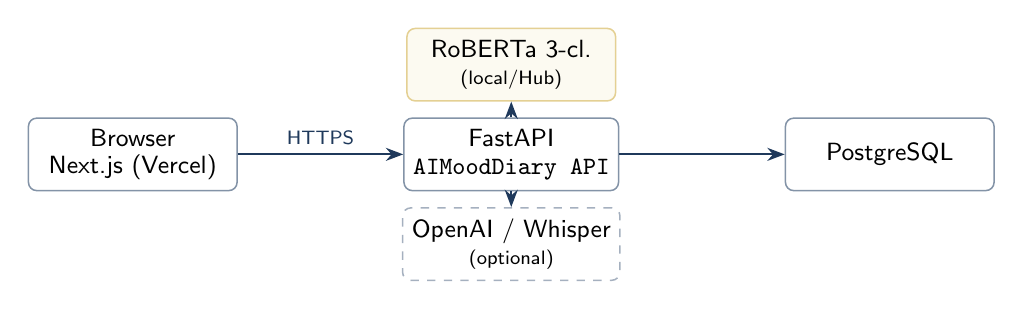
\begin{tikzpicture}[
  node distance=0.9cm and 1.0cm,
  box/.style={draw=MMnavy!55, line width=0.55pt, fill=white, rounded corners=3pt,
    align=center, minimum width=2.65cm, minimum height=0.92cm, font=\small\sffamily},
  small/.style={font=\scriptsize\sffamily\color{MMnavyL!85}},
  arr/.style={-{Stealth[length=2.2mm]}, thick, color=MMnavyL!70!black}
]
\node[box] (fe) {Browser\\[-1pt]{\small Next.js (Vercel)}};
\node[box, right=2.1cm of fe] (api) {{\small FastAPI}\\[-1pt]\texttt{AIMoodDiary API}};
\node[box, right=2.1cm of api] (db) {{\small PostgreSQL}};
\node[box, above=0.2cm of api, fill=MMgoldL!12, draw=MMgold!50] (hf) {RoBERTa 3-cl.\\[-1pt]{\scriptsize (local/Hub)}};
\node[box, below=0.2cm of api, draw=MMnavy!40, dashed] (oa) {OpenAI / Whisper\\[-1pt]{\scriptsize (optional)}};

\draw[arr] (fe) -- node[above, small] {HTTPS} (api);
\draw[arr] (api) -- (db);
\draw[arr] (api) -- (hf);
\draw[arr, dashed] (api) -- (oa);
\end{tikzpicture}
\caption{High-level architecture: the SPA talks to the API; the API runs inference and storage; OpenAI is used for diary and speech if configured.}
\label{fig:arch}
\end{figure}

%==============================================================================
\section{Methodology and data}
The \textbf{GoEmotions} dataset (HuggingFace) is used in the legacy pipeline, with 54{,}263 samples; labels are reduced to 7 and then 3 classes (\texttt{negative}, \texttt{neutral}, \texttt{positive}) for the product model. Baselines in research include \textbf{Logistic Regression + TF-IDF}, \textbf{DistilBERT}, and \textbf{RoBERTa} (7- and 3-class). The production backend uses the \textbf{3-class RoBERTa} with a label mapping in JSON (IDs $0$/$1$/$2$ $\rightarrow$ negative/neutral/positive).

%==============================================================================
\section{Implementation details and code snippets}
\label{sec:impl}

\subsection{Emotion label mapping (3-class)}
\begin{tcblisting}{
  listing only,
  title={\texttt{backend/app/assets/emotion\_mapping\_3class.json}},
  colbacktitle=codebg,
  coltitle=MMnavyL!90!black,
  fonttitle=\ttfamily\footnotesize,
  colback=codebg,
  colframe=codeframe,
  boxrule=0.7pt,
  arc=1.5pt,
  top=0.12em, bottom=0.15em,
  listing options={
    language=json,
    basicstyle=\ttfamily\footnotesize,
    stringstyle=\color{str},
    breaklines=true,
    columns=fullflexible,
  }
}
{
  "emotion_to_id": {
    "negative": 0,
    "neutral": 1,
    "positive": 2
  }
}
\end{tcblisting}
\noindent\small\color{MMnavyL!80!black} Valid JSON as stored in the repository.

\subsection{Classifier forward pass (excerpt)}
The service tokenizes, runs the transformer, and applies softmax. The class with highest probability is the prediction; confidence is that probability.

\begin{tcblisting}{listing only, listing options={style=mmcode},
  colback=codebg, colframe=codeframe, boxrule=0.7pt, arc=1.5pt, top=0.15em, bottom=0.2em, left=0.12em,
  before upper={\CodeFilename{emotion\_classifier.py (excerpt)}}
}
def predict(self, text: str) -> EmotionPrediction:
    text = (text or "").strip()
    if not text:
        raise ValueError("Text must be non-empty.")
    enc = self._tokenizer(
        text, truncation=True, padding="max_length",
        max_length=self.max_length, return_tensors="pt",
    )
    enc = {k: v.to(self._device) for k, v in enc.items()}
    with torch.no_grad():
        logits = self._model(**enc).logits
        probs_t = torch.softmax(logits, dim=-1)[0].detach().cpu()
    # ... map indices to label strings, pick argmax ...
    return EmotionPrediction(
        label=best_label, confidence=confidence, probabilities=probs
    )
\end{tcblisting}

\subsection{Prediction API contract}
\begin{tcblisting}{listing only, listing options={style=mmcode},
  colback=codebg, colframe=codeframe, boxrule=0.7pt, arc=1.5pt, top=0.15em, bottom=0.2em,
  before upper={\CodeFilename{app/api/routes/predict.py (excerpt)}}
}
class PredictRequest(BaseModel):
    text: str = Field(..., min_length=1, max_length=10_000)

class PredictResponse(BaseModel):
    label: str
    confidence: float
    probabilities: dict[str, float]
\end{tcblisting}
Batch variant accepts up to 128 strings (\texttt{PredictBatchRequest}).

\subsection{Diary: LLM prompt guardrails (excerpt)}
The diary is generated so that the model \emph{only} uses user keywords, reducing hallucinated events; tone is optional.
\begin{tcblisting}{listing only, listing options={style=mmcode},
  colback=codebg, colframe=codeframe, boxrule=0.7pt, arc=1.5pt, top=0.15em, bottom=0.2em,
  before upper={\CodeFilename{llm\_service.py (excerpt)}}
}
def generate_diary(self, keywords: str, tone: Optional[str] = None) -> str:
    tone_part = f"in a {tone} tone" if tone else "in a natural tone"
    prompt = (
        "You are helping a user write a short daily diary entry.\n\n"
        "RULES (follow strictly):\n"
        "- Use ONLY the ideas, events, and feelings mentioned in the keywords below. "
        "Do NOT add any events, activities, places, or details (e.g. walks, sunshine, coffee, friends) that are not in the keywords.\n"
        "- If the user gives only 1-2 keywords, write a very short entry (1-3 sentences)...\n"
        f"- Write in first person, {tone_part}. Be concise.\n\n"
        f"Keywords (use these only): {keywords}\n\n"
        "Diary:"
    )
    response = self._client.chat.completions.create(
        model=self._model_name,
        messages=[{"role": "user", "content": prompt}],
    )
    if response.choices and response.choices[0].message.content:
        return response.choices[0].message.content.strip()
    return ""
\end{tcblisting}

\subsection{Diary: blending classifier scores}
After the LLM returns text, the API predicts on \textbf{keywords} and on the \textbf{generated diary} separately, then blends: \textbf{72\%} keyword probabilities + \textbf{28\%} diary probabilities, followed by a lexical \textbf{calibration} step (\texttt{diary\_sentiment\_calibration.py}) to reduce spurious \emph{positive} bias from silver-lining phrasing on stressful content.

%==============================================================================
\section{Insights engine (summary)}
\label{sec:insights-engine}

The \texttt{PatternEngine} requires minimum entry counts: \textbf{3} for trend/keywords, \textbf{7} for weekday rhythm, \textbf{5} for transition / next-day style statistics. It outputs trend slope and direction, weekly scores, volatility, a transition matrix with a \textbf{70\%}/\textbf{30\%} Markov/recent-day blend, keyword correlations, streaks, and short natural-language \texttt{insights} lines. Crisis-related tokens are handled carefully so that harmful keywords are not presented as \emph{positive} correlates.

\noindent\textit{Example UI charts for Insights are in \S\ref{sec:ui-figs} (Figures~\ref{fig:app-insights-trend} and~\ref{fig:app-insights-extras}).}

%==============================================================================
\section{Results and visualizations (legacy + product)}
\label{sec:results-figs}

\noindent
\textbf{Recommended legacy assets to export into Overleaf:}
\begin{itemize}[itemsep=0.3em,label=\color{MMnavy}$\bullet$]
  \item \textbf{Model comparison:} \texttt{legacy/results/models/model\_comparison.csv} (or equivalent after running \texttt{model\_evaluation.py}) $\rightarrow$ table or bar chart in \LaTeX.
  \item \textbf{Confusion matrices:} PNGs from \texttt{legacy/results/figures/} (one per model or per best model; prioritize \textbf{RoBERTa 3-class} to match production).
  \item \textbf{Data exploration:} e.g.\ \texttt{emotion\_distribution.png} (if your notebook saved it) for dataset section.
  \item \textbf{Streamlit:} one screenshot of the live prediction page for the ``before product'' story.
\end{itemize}

% --- Subfig (a): EXPECTED figures/legacy-02-confusion-3cl.png | (b): EXPECTED figures/legacy-03-emotion-distribution.png
\begin{figure}[H]
  \centering
  \begin{subfigure}[b]{0.48\textwidth}
    \centering
%   \includegraphics[width=\linewidth,keepaspectratio]{figures/legacy-02-confusion-3cl.png}
    \MMPending{figures/legacy-02-confusion-3cl.png}{Export from \texttt{legacy/results/figures/} after evaluation; use the RoBERTa 3-class matrix.}
    \caption{Confusion matrix (3-class).}
    \label{fig:legacy-conf}
  \end{subfigure}
  \hfill
  \begin{subfigure}[b]{0.48\textwidth}
    \centering
%   \includegraphics[width=\linewidth,keepaspectratio]{figures/legacy-03-emotion-distribution.png}
    \MMPending{figures/legacy-03-emotion-distribution.png}{From data exploration or training notebook (e.g.\ \texttt{emotion\_distribution.png}).}
    \caption{Label distribution (example).}
    \label{fig:legacy-dist}
  \end{subfigure}
  \caption{Legacy pipeline: evaluation and data exploration. File names: \texttt{legacy-02-confusion-3cl.png}, \texttt{legacy-03-emotion-distribution.png}.}
  \label{fig:legacy-pair}
\end{figure}

% --- EXPECTED FILE: figures/legacy-01-streamlit.png
\begin{figure}[H]
  \centering
%  \includegraphics[width=0.85\textwidth,keepaspectratio]{figures/legacy-01-streamlit.png}
  \MMPending{figures/legacy-01-streamlit.png}{Streamlit window: text input and predicted emotion with confidence.}
  \caption{Legacy Streamlit demo (\texttt{legacy-01-streamlit.png}).}
  \label{fig:legacy-streamlit}
\end{figure}

\noindent\textit{Product UI close-ups also appear in \S\ref{sec:ui-figs}.}

%==============================================================================
\section{Challenges and mitigations (selected)}
\begin{itemize}[itemsep=0.3em, label=\sffamily\color{MMnavy}$\triangleright$]
  \item \textbf{LLM optimism:} 72/28 blend + post-hoc calibration on lexicon of stress/negative cues.
  \item \textbf{Domain gap:} GoEmotions training vs student language; document as a limitation; 3 classes align with simple product UX.
  \item \textbf{Analytics safety:} crisis-token handling in keyword correlation outputs.
  \item \textbf{Lightweight API bundle:} \texttt{hf-deploy/} omits optional routes (e.g.\ speech, minigames) for lean hosting; full stack lives under \texttt{backend/}.
\end{itemize}

%==============================================================================
\section{Conclusion and future work}
AIMoodDiary delivers an integrated path from \textbf{research} (GoEmotions, baselines, Streamlit) to a \textbf{deployed} Next.js and FastAPI product with a clear GitHub home: \url{https://github.com/manumathewjiss/moodmirror-student-wellness-tracker/tree/main}. Future work may include in-domain data collection, smaller on-device models, and multilingual support, subject to privacy and duty-of-care review.

%==============================================================================
\appendix
\section{Quick checklist (file names)}

\noindent
Upload these to \texttt{figures/} (see Table~\ref{tab:figure-files} for what each should show). For each figure: uncomment the matching \texttt{\textbackslash includegraphics} line and remove the PENDING box (as in the \texttt{SETUP} block at the top of this file).
\begin{itemize}[itemsep=0.2em, leftmargin=1.1em, label={—}]
  \item \textbf{App (tabs):} \texttt{app-01-home.png} through \texttt{app-10-unwind.png}
  \item \textbf{Legacy:} \texttt{legacy-01-streamlit.png}, \texttt{legacy-02-confusion-3cl.png}, \texttt{legacy-03-emotion-distribution.png}
\end{itemize}

\end{document}
